\documentclass{article}
\usepackage{amsmath}
\usepackage{tikz}
\usetikzlibrary{arrows.meta}

\begin{document}

\begin{figure}[h]
    \centering
    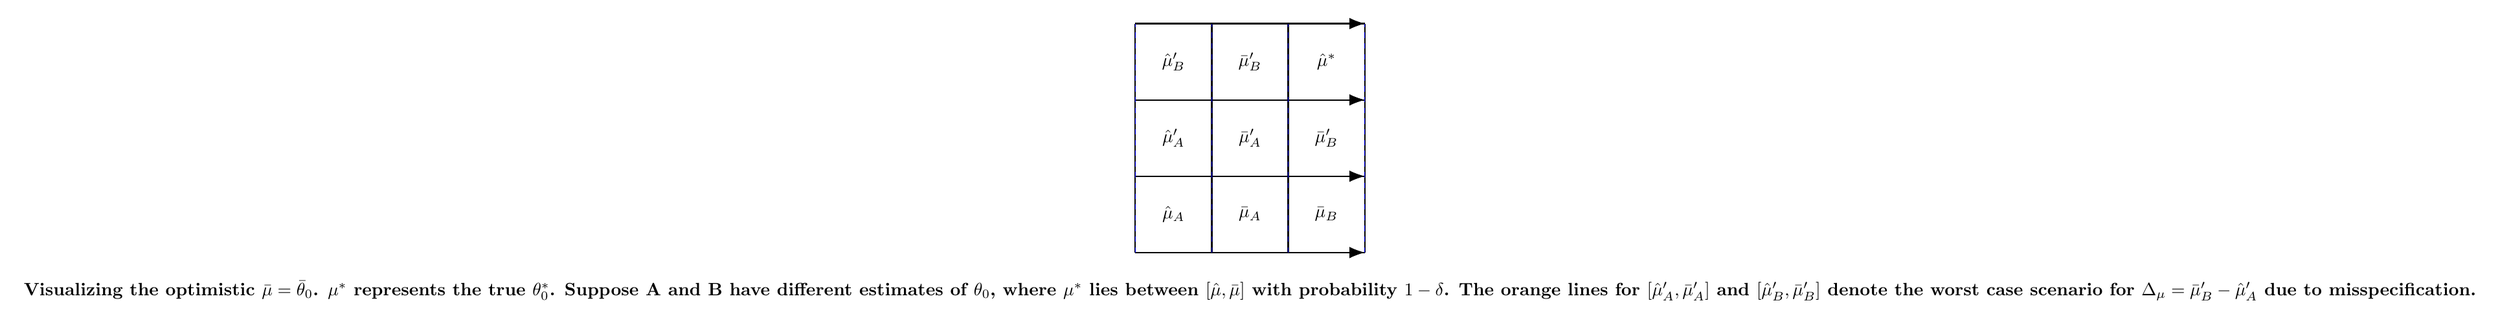
\begin{tikzpicture}[scale=1.5]
        % Draw the horizontal lines
        \draw[thick] (0,0) -- (3,0);
        \draw[thick] (0,1) -- (3,1);
        \draw[thick] (0,2) -- (3,2);
        \draw[thick] (0,3) -- (3,3);

        % Draw the vertical lines
        \draw[thick] (0,0) -- (0,3);
        \draw[thick] (1,0) -- (1,3);
        \draw[thick] (2,0) -- (2,3);
        \draw[thick] (3,0) -- (3,3);

        % Draw the arrows
        \draw[-{Latex[length=3mm]}] (0,0) -- (3,0);
        \draw[-{Latex[length=3mm]}] (0,1) -- (3,1);
        \draw[-{Latex[length=3mm]}] (0,2) -- (3,2);
        \draw[-{Latex[length=3mm]}] (0,3) -- (3,3);

        % Label the points
        \node at (0.5, 0.5) {$\hat{\mu}_A$};
        \node at (1.5, 0.5) {$\bar{\mu}_A$};
        \node at (2.5, 0.5) {$\bar{\mu}_B$};
        \node at (0.5, 1.5) {$\hat{\mu}_A'$};
        \node at (1.5, 1.5) {$\bar{\mu}_A'$};
        \node at (2.5, 1.5) {$\bar{\mu}_B'$};
        \node at (0.5, 2.5) {$\hat{\mu}_B'$};
        \node at (1.5, 2.5) {$\bar{\mu}_B'$};
        \node at (2.5, 2.5) {$\hat{\mu}^*$};

        % Dashed line
        \draw[dashed, blue] (0,0) -- (0,3);
        \draw[dashed, blue] (1,0) -- (1,3);
        \draw[dashed, blue] (2,0) -- (2,3);
        \draw[dashed, blue] (3,0) -- (3,3);

        % Caption
        \node at (1.5, -0.5) {\textbf{Visualizing the optimistic $\bar{\mu} = \bar{\theta}_0$. $\mu^*$ represents the true $\theta_0^*$. Suppose A and B have different estimates of $\theta_0$, where $\mu^*$ lies between $[\hat{\mu}, \bar{\mu}]$ with probability $1 - \delta$. The orange lines for $[\hat{\mu}_A', \bar{\mu}_A']$ and $[\hat{\mu}_B', \bar{\mu}_B']$ denote the worst case scenario for $\Delta_{\mu} = \bar{\mu}_B' - \hat{\mu}_A'$ due to misspecification.}};
    \end{tikzpicture}
\end{figure}

\end{document}